
\begin{exercise}

% !TEX root = ../main.tex



 Een buffel tracht loodrecht een $300\rm\,m$ brede rivier over te steken met een snelheid van $1,00\rm\,m/s$. Als de stroomsnelheid $1,50\rm\,m/s$ is, in welke tijd bereikt hij dan de overzijde en hoe ver zal hij afgedreven zijn? Construeer de snelheidsvectoren en bereken de grootte van de resulterende snelheid.
\begin{oplossing}
\item[\textit{Gegeven}]$d=300\rm\,m$, $v_y=1,00\rm\,m/s$, $v_x=1,50\rm\,m/s$.
\item[\textit{Gevraagd}]$t$, $x$, $v$
\item[\textit{Oplossing}]De snelheden worden in onderstaande figuur weergegeven.
\begin{figure}[h]
\begin{center}
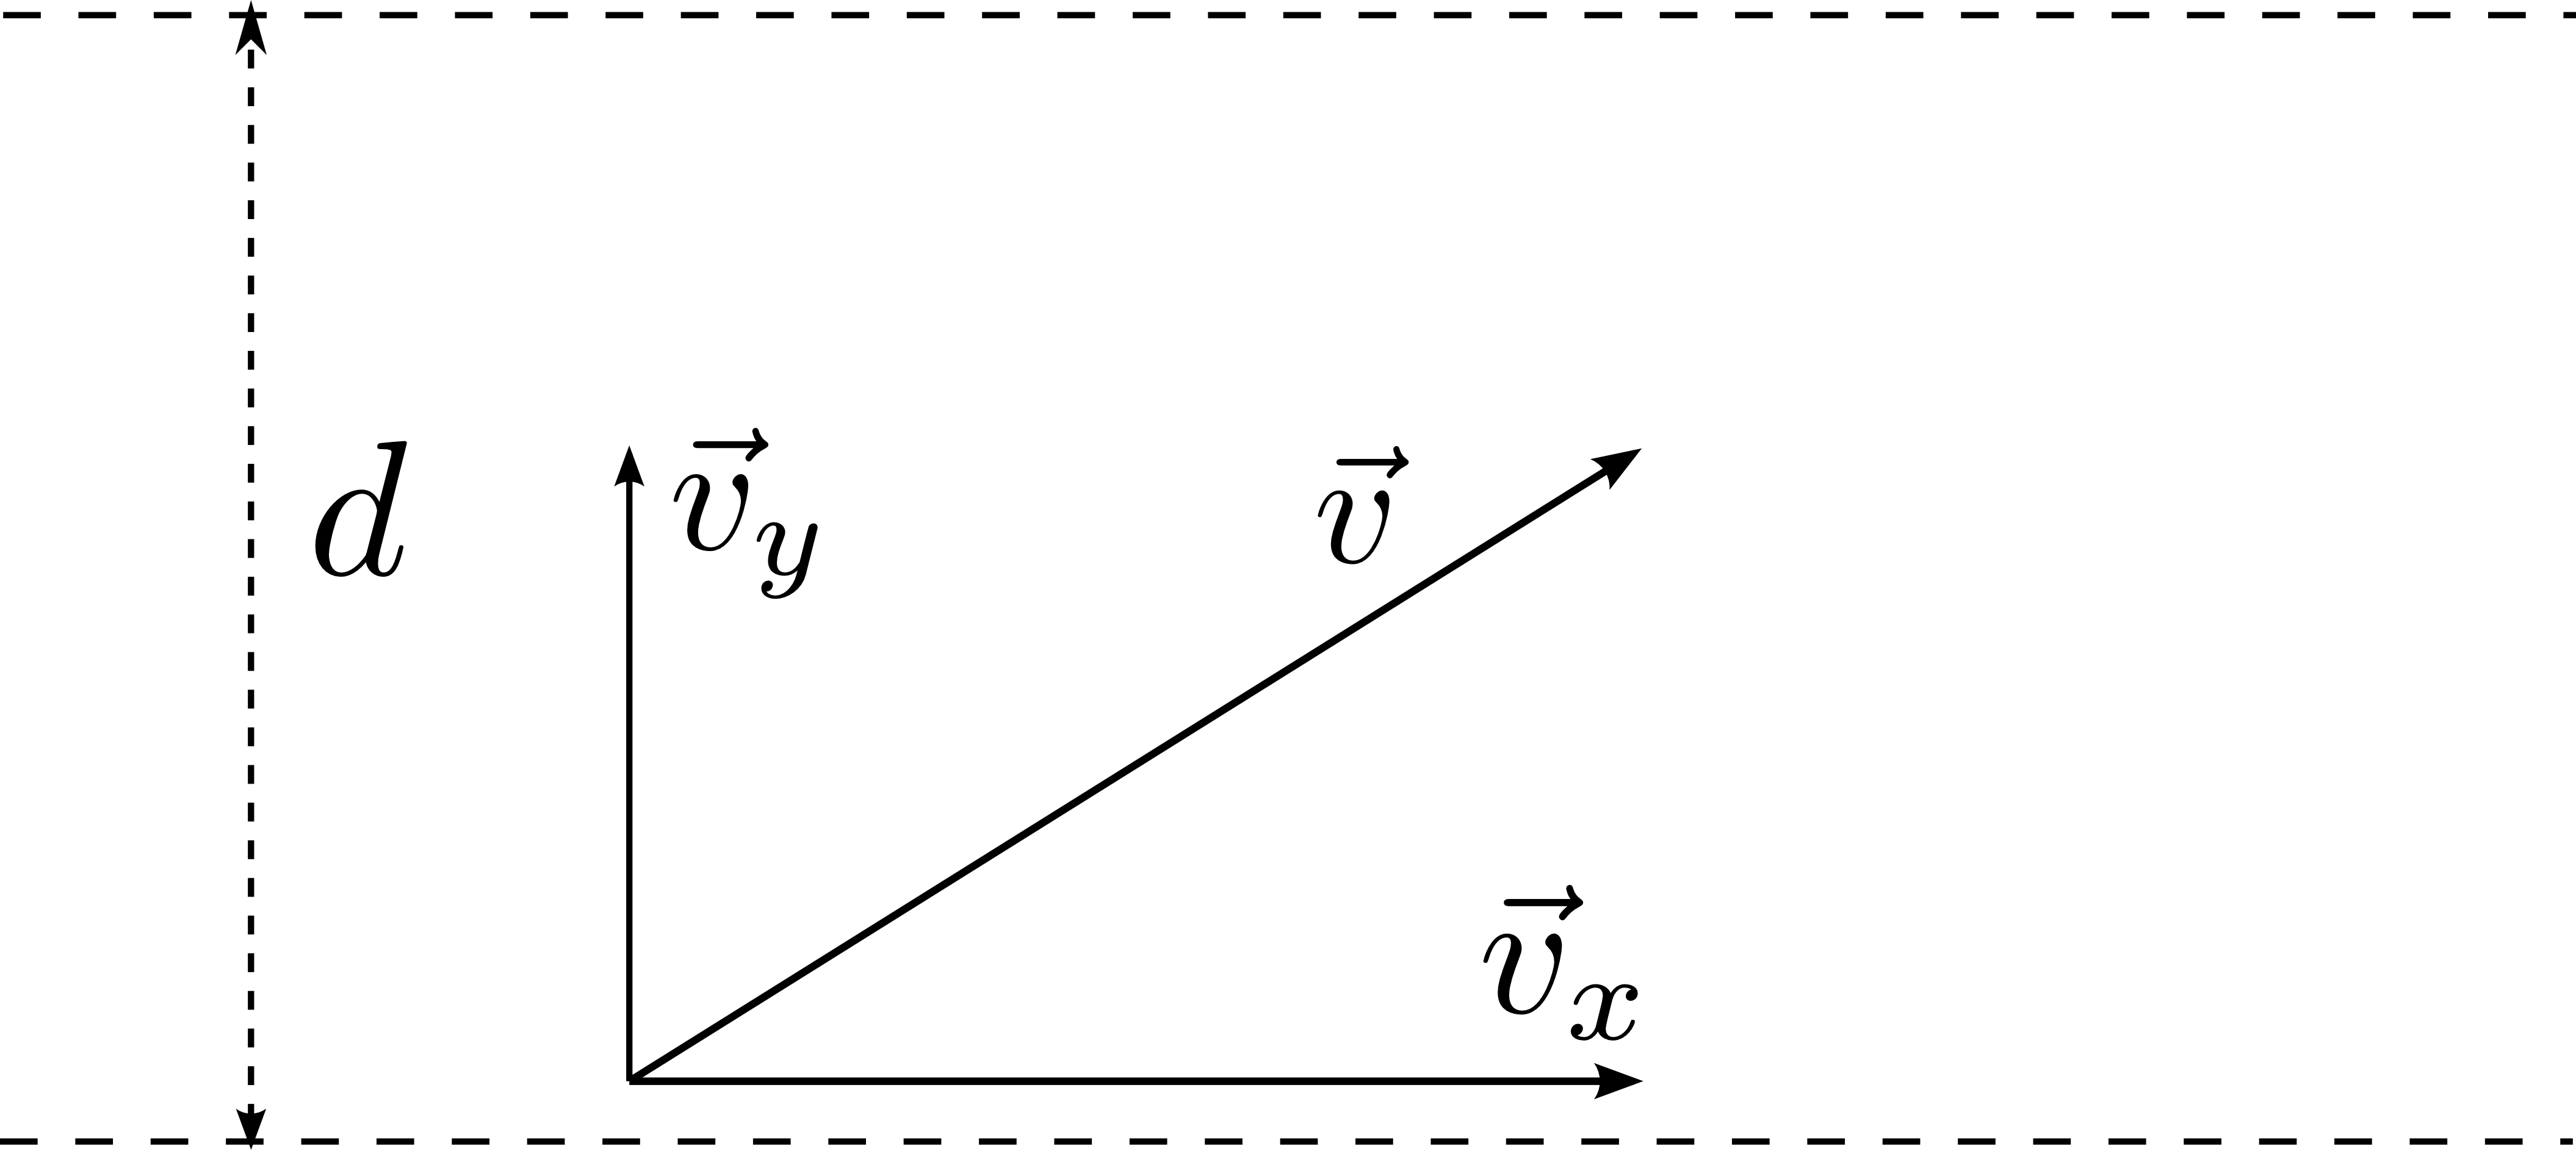
\includegraphics[width=0.7\textwidth]{dyn/exercises/4p49}
\end{center}
\end{figure}
De tijd die nodig is om de overkant te bereiken vinden we eenvoudigweg door de afstand te delen door de snelheid die de buffel loodrecht op oever heeft. De snelheid van de stroming heeft hierop immers geen invloed.
\begin{eqnarray*}
t=\frac{d}{v_y}=300\rm\,s
\end{eqnarray*}
Gedurende die tijd is hij door de stroming meegevoerd zodat we de afstand die hij is afgedreven kunnen berekenen als volgt.
\begin{eqnarray*}
x=v_xt=450\rm\,m
\end{eqnarray*}
De grootte van de resulterende snelheid vinden we met de stelling van Pythagoras: $v=\sqrt{v_x^2+v_y^2}=1,8\rm\,m/s$.
\end{oplossing}

\end{exercise}
